\section{Resilience test}

The resilience analysis follows two distinct metodologies, where we test first static failures and then dynamical overload
cascades. In both cases the observable is the
relative size of the largest connected component (LCC): a small LCC means that
the surviving nodes are fragmented and can no longer
provide a connected network.


Four different strategies for the static failure test are implemented: random failure and three types of targeted attacks.
In random failure, a fraction $p_{\mathrm{fail}}$ of nodes is selected randomly and removed. For targeted attacks, nodes are instead ranked and removed once by
degree, then by betweenness centrality, and finally by $k$-coreness. The first targets well-connected nodes, the second targets nodes important for
shortest-path traffic, and the third looks at nodes in the innermost shells of
the core decomposition, testing how dependent is the network on its structurally deepest core. We record $S(p_{\mathrm{fail}})/N$, the relative LCC
size, as a function of the surviving-node fraction
$1-p_{\mathrm{fail}}$.




The cascade experiment uses the Motter--Lai model. Each node $i$ has a fixed
capacity $C_i$ and a dynamic load $L_i(\tau)$. The load is estimated as the
betweenness centrality of node $i$: it measures how often shortest paths traverse that node, and it is recomputed on the
surviving network after each generation. If the new load exceeds a node's capacity, that node fails and may
trigger a further redistribution in the network.
The initial attack removes the highest-degree node of the LCC. We set the
baseline capacity to the initial load, $C_i=L_i(0)$, and scale it to
$(1+\alpha)C_i$, where $\alpha$ is the capacity-tolerance parameter. At every
generation all nodes satisfying $L_i>(1+\alpha)C_i$ are removed. The process
ends when no overload remains. 
Each cascade uses a fixed cohort of 128 source nodes to estimate node betweenness centralities. In practice, 
for each source, shortest paths to all surviving nodes are considered, and the load of a node $i$ is related to how often it lies on these paths. The correct procedure would be to calculate the betweeness by looping
over all the possible pairs of nodes in the network, but we avoided this procedure to gain more computational efficiency. \\
Therefore, we repeat the experiment for three synthetic-network realizations
and three independent cohorts per realization. The final result reports only the mean
final LCC over these nine runs. 


\begingroup\scriptsize

\begin{figure}[H]
\centering
\begin{minipage}{.47\linewidth}\centering
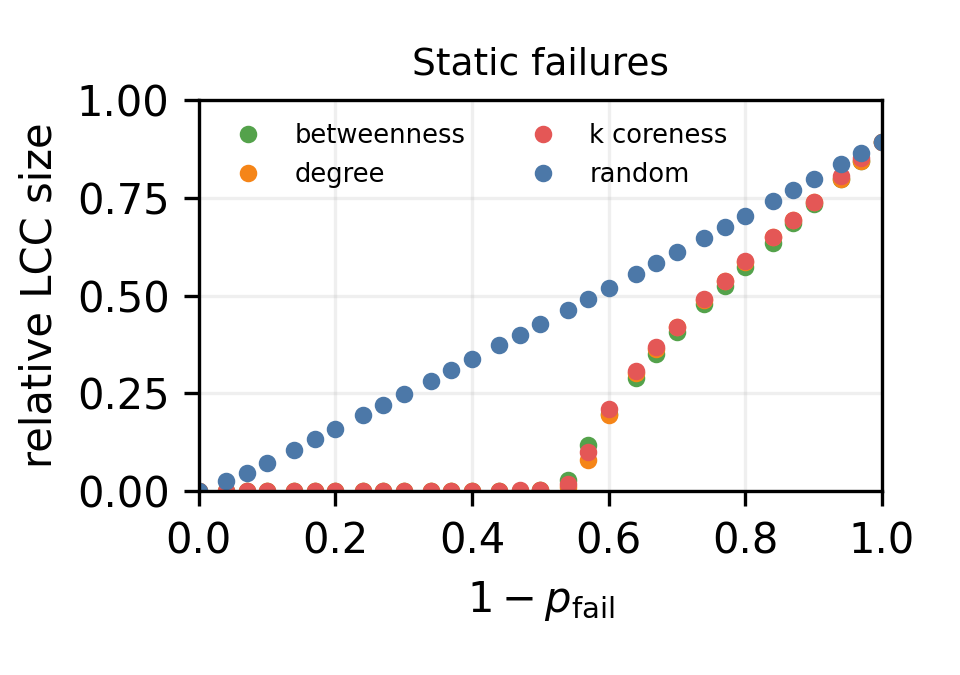
\includegraphics[width=\linewidth]{results/analysis_seed42/static_failures.png}
\end{minipage}\hfill
\begin{minipage}{.47\linewidth}\centering
\IfFileExists{results/analysis_ensemble/cascade_ensemble_mean.png}{%
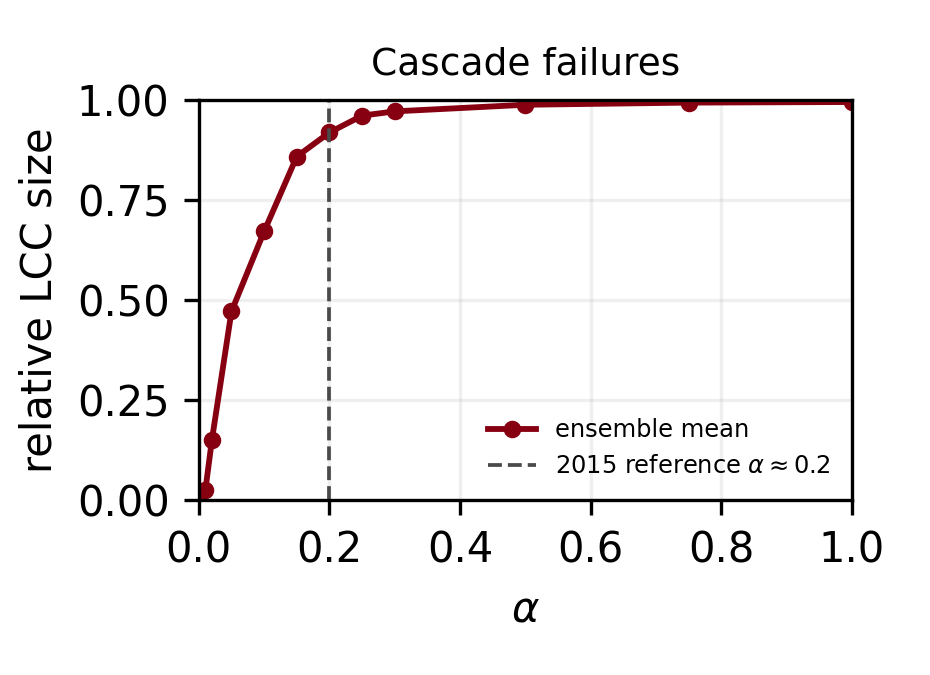
\includegraphics[width=\linewidth]{results/analysis_ensemble/cascade_ensemble_mean.png}%
}{\fbox{\parbox[c][1.4in][c]{.9\linewidth}{\centering Cascade sweep pending.}}}
\end{minipage}
\caption{Synthetic-network resilience results.}
\label{fig:darknet-resilience}
\end{figure}

\endgroup

As regards static failures, fig.~\ref{fig:darknet-resilience} shows that the synthetic graph is more vulnerable to targeted than
to random removal, but its targeted fragmentation occurs only near
$p_{\mathrm{fail}}\simeq0.45$, equivalently
$1-p_{\mathrm{fail}}\simeq0.55$. This is qualitatively consistent with the empirical reference result $1-p_{\mathrm{fail}}\simeq0.6$. Instead, for cascade failures, fig.~\ref{fig:darknet-resilience} reports the final LCC fraction over a sweep of $12$ values of $\alpha$.
Our synthetic network remains fully operative after $\alpha\simeq0.3$, which is in good agreement with the empirical
reference $\alpha\simeq0.2$. Yet, even for lower values of $\alpha$ the network is still not too much fragmented, for example the LCC relative size is $0.5$ for $\alpha=0.05$.
